% ===================================================================
%  Week 5 — Session 1: Gradients & derivative operators
% ===================================================================
\documentclass[10pt,aspectratio=169]{beamer}
% ===================================================================
%  Shared Beamer preamble for "Practical Image Processing"
%  English slides. Compile with pdfLaTeX.
% ===================================================================

\usetheme{metropolis}
\usepackage[T1]{fontenc}
\usepackage[utf8]{inputenc}
\usepackage{lmodern}
\usepackage{listings}
\usepackage{tcolorbox}
\usepackage{fontawesome5}
\usepackage{booktabs}
\usepackage{amsmath,amssymb}
\usepackage{tikz}
\usepackage{pgfplots}
\pgfplotsset{compat=1.17}
\usetikzlibrary{arrows.meta,positioning,shapes.geometric,fit,backgrounds,matrix}
\tcbuselibrary{skins,breakable}

% ---- Palette --------------------------------------------------------
\definecolor{coursePrimary}{HTML}{1B4965}   % deep blue
\definecolor{courseAccent}{HTML}{E76F51}    % coral
\definecolor{courseGood}{HTML}{2A9D8F}      % teal
\definecolor{courseBad}{HTML}{C0392B}       % red
\definecolor{courseInfo}{HTML}{2980B9}      % blue
\definecolor{codeBg}{HTML}{F5F6FA}
\definecolor{codeKw}{HTML}{8E44AD}
\definecolor{codeStr}{HTML}{2A9D8F}
\definecolor{codeCom}{HTML}{7F8C8D}

\setbeamercolor{frametitle}{bg=coursePrimary}
\setbeamercolor{progress bar}{fg=courseAccent}
\setbeamercolor{alerted text}{fg=courseAccent}
\metroset{block=fill,sectionpage=progressbar,numbering=fraction}

% ---- Code listings (Python is built into listings) -----------------
\lstdefinestyle{course}{
  backgroundcolor=\color{codeBg},
  basicstyle=\ttfamily\scriptsize,
  keywordstyle=\color{codeKw}\bfseries,
  stringstyle=\color{codeStr},
  commentstyle=\color{codeCom}\itshape,
  numberstyle=\tiny\color{codeCom},
  numbers=left, numbersep=6pt,
  showstringspaces=false, breaklines=true, breakatwhitespace=true,
  tabsize=4, columns=fullflexible,
  frame=single, framesep=4pt, rulecolor=\color{gray!30},
  keepspaces=true, upquote=true, language=Python,
}
\lstset{style=course}
\lstdefinelanguage{bash}{
  keywords={cd,pip,python,venv,source,import}, sensitive=true,
  morecomment=[l]{\#}, morestring=[b]', morestring=[b]",
}

% ---- Reusable callout boxes ----------------------------------------
\newtcolorbox{goodbox}[1][Good practice]{colback=courseGood!8,colframe=courseGood,
  fonttitle=\bfseries,title={\faCheck~#1},boxrule=0.6pt,left=4pt,right=4pt,top=3pt,bottom=3pt}
\newtcolorbox{badbox}[1][Pitfall]{colback=courseBad!8,colframe=courseBad,
  fonttitle=\bfseries,title={\faTimes~#1},boxrule=0.6pt,left=4pt,right=4pt,top=3pt,bottom=3pt}
\newtcolorbox{infobox}[1][Note]{colback=courseInfo!8,colframe=courseInfo,
  fonttitle=\bfseries,title={\faInfoCircle~#1},boxrule=0.6pt,left=4pt,right=4pt,top=3pt,bottom=3pt}
\newtcolorbox{mathbox}[1][Math]{colback=coursePrimary!6,colframe=coursePrimary,
  fonttitle=\bfseries,title={\faCalculator~#1},boxrule=0.6pt,left=4pt,right=4pt,top=3pt,bottom=3pt}

\newcommand{\keyidea}[1]{\begin{alertblock}{Key idea}#1\end{alertblock}}
\newcommand{\term}[1]{\textbf{\color{coursePrimary}#1}}
\newcommand{\code}[1]{\lstinline[basicstyle=\ttfamily\small]|#1|}

% ---- A helper to draw a small pixel grid, cells shaded by value ----
% \pixelgrid{ {10,20,120,200,240}, {30,60,130,180,230}, ... }
\newcommand{\pixelgrid}[1]{%
  \begin{tikzpicture}[font=\scriptsize,scale=0.6]
    \foreach \row [count=\ry] in {#1} {
      \foreach \val [count=\cx] in \row {
        \draw[gray,fill=coursePrimary!8] (\cx,-\ry) rectangle ++(1,-1);
        \node at (\cx+0.5,-\ry-0.5) {\val};
      }
    }
  \end{tikzpicture}}


\title{Edge Detection}
\subtitle{Week 5 — Session 1: Gradients \& derivative operators}
\author{Practical Image Processing}
\date{Lecture 5.1 \textbullet\ 60--70 min}

\begin{document}

\maketitle

\begin{frame}{Recap \& today}
  \begin{columns}[T]
    \begin{column}{0.58\textwidth}
      \begin{itemize}
        \item Wk3--4: smoothing/denoising with kernels — killing \term{high frequencies}.
        \item \alert{Today (Session 1):} \term{edges} — where intensity changes sharply.
              We treat an edge as a large \term{derivative} and build the classic
              gradient operators (Sobel, Prewitt, Scharr, Laplacian/LoG).
        \item Next session: assemble these into the \term{Canny} detector.
      \end{itemize}
    \end{column}
    \begin{column}{0.42\textwidth}
      \begin{alertblock}{DocScan milestone}
        Finding the page/meter boundary starts with edges. This week's output feeds the
        ``find the page'' step later in the course.
      \end{alertblock}
    \end{column}
  \end{columns}
\end{frame}

\begin{frame}{Roadmap — Session 1}\tableofcontents\end{frame}

% ==================================================================
\section{What is an edge?}
% ==================================================================

\begin{frame}{An edge = a rapid intensity change}
  \begin{itemize}
    \item Where the image jumps from dark to light (or vice versa) — object boundaries, text strokes.
    \item Mathematically, a large \term{gradient}: the derivative of intensity is high there.
    \item Edges are \term{high-frequency} (Week 3) — so we detect them with a high-pass kernel.
  \end{itemize}
  \begin{mathbox}
    Gradient $\nabla f = (f_x, f_y)$; magnitude $|\nabla f| = \sqrt{f_x^2 + f_y^2}$;
    direction $\theta=\operatorname{atan2}(f_y,f_x)$.
  \end{mathbox}
\end{frame}

\begin{frame}{A 1D edge and its derivative}
  \begin{columns}[T]
    \begin{column}{0.5\textwidth}
      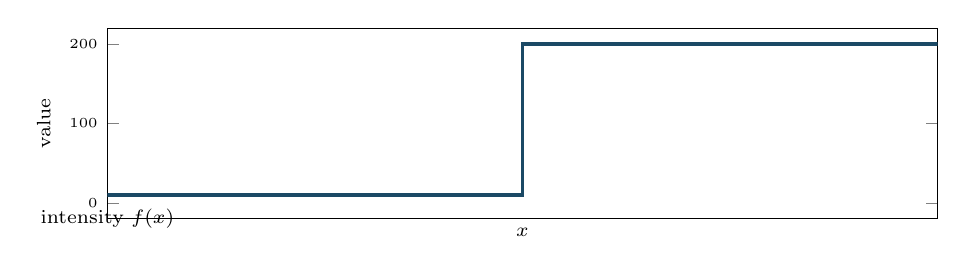
\begin{tikzpicture}
        \begin{axis}[width=\linewidth,height=4cm,title={intensity $f(x)$},
          xlabel={$x$},ylabel={value},ymin=-20,ymax=220,xmin=0,xmax=6,
          xtick=\empty,every axis title/.style={font=\scriptsize},
          label style={font=\scriptsize},tick label style={font=\tiny}]
          \addplot[coursePrimary,very thick,const plot] coordinates
            {(0,10)(1,10)(2,10)(3,200)(4,200)(5,200)(6,200)};
        \end{axis}
      \end{tikzpicture}
    \end{column}
    \begin{column}{0.5\textwidth}
      \begin{tikzpicture}
        \begin{axis}[width=\linewidth,height=4cm,title={derivative $f'(x)$},
          xlabel={$x$},ylabel={value},ymin=-20,ymax=220,xmin=0,xmax=6,
          xtick=\empty,every axis title/.style={font=\scriptsize},
          label style={font=\scriptsize},tick label style={font=\tiny}]
          \addplot[courseAccent,very thick,ycomb,mark=*,mark size=1pt] coordinates
            {(1,0)(2,0)(3,190)(4,0)(5,0)};
        \end{axis}
      \end{tikzpicture}
    \end{column}
  \end{columns}
  \vspace{2pt}
  \keyidea{The edge is exactly where the derivative spikes. ``Find edges'' $=$ ``find large derivatives''.}
\end{frame}

\begin{frame}{Four edge profiles you will meet}
  \begin{center}
  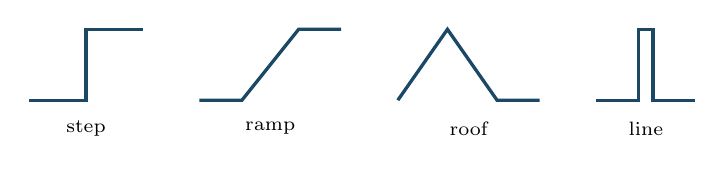
\begin{tikzpicture}[font=\scriptsize,scale=0.9]
    % step
    \draw[coursePrimary,very thick] (0,0)--(0.8,0)--(0.8,1)--(1.6,1);
    \node at (0.8,-0.4){step};
    % ramp
    \draw[coursePrimary,very thick] (2.4,0)--(3.0,0)--(3.8,1)--(4.4,1);
    \node at (3.4,-0.4){ramp};
    % roof
    \draw[coursePrimary,very thick] (5.2,0)--(5.9,1)--(6.6,0)--(7.2,0);
    \node at (6.2,-0.4){roof};
    % line
    \draw[coursePrimary,very thick] (8.0,0)--(8.6,0)--(8.6,1)--(8.8,1)--(8.8,0)--(9.4,0);
    \node at (8.7,-0.4){line};
  \end{tikzpicture}
  \end{center}
  \begin{itemize}
    \item \term{Step}: ideal boundary. \term{Ramp}: a blurred/soft edge (real optics).
    \item \term{Roof}/\term{line}: thin structures — a stroke of text, a wire, a meter needle.
    \item First derivative peaks at steps/ramps; a thin \term{line} shows up as a \emph{pair} of opposite peaks.
  \end{itemize}
\end{frame}

% ==================================================================
\section{First derivative: gradient operators}
% ==================================================================

\begin{frame}{Derivatives as kernels}
  \begin{columns}[T]
    \begin{column}{0.5\textwidth}
      \term{Sobel-x} (vertical edges):
      \[\begin{bmatrix}-1&0&1\\-2&0&2\\-1&0&1\end{bmatrix}\]
    \end{column}
    \begin{column}{0.5\textwidth}
      \term{Sobel-y} (horizontal edges):
      \[\begin{bmatrix}-1&-2&-1\\0&0&0\\1&2&1\end{bmatrix}\]
    \end{column}
  \end{columns}
  \vspace{4pt}
  Each computes a \emph{difference} across the pixel — a discrete derivative. Weights sum to 0,
  so a flat region gives 0, exactly as an edge kernel should.
  \begin{infobox}[Separable]
    Sobel-x $=$ smoothing column $[1,2,1]^{\!\top}$ times differencing row $[-1,0,1]$: blur one
    axis, difference the other. That is why Sobel is a \emph{denoised} derivative.
  \end{infobox}
\end{frame}

\begin{frame}{Worked example: Sobel-x on a patch}
  A $3\times3$ neighbourhood (a dark-to-light vertical edge):
  \begin{columns}[T]
    \begin{column}{0.42\textwidth}
      \begin{center}
      \pixelgrid{ {10,10,200}, {10,10,200}, {10,10,200} }
      \end{center}
    \end{column}
    \begin{column}{0.58\textwidth}
      \small
      \begin{align*}
        g_x &= (-1)(10)+(1)(200)\\
            &\quad +(-2)(10)+(2)(200)\\
            &\quad +(-1)(10)+(1)(200)\\
            &= 4(200-10) = \mathbf{760}
      \end{align*}
      A big positive response: a strong vertical edge, dark$\to$light left to right.
    \end{column}
  \end{columns}
  \vspace{2pt}
  \begin{goodbox}
    Sign carries direction: a light$\to$dark edge would give $-760$. Take $|g_x|$ for an
    ``edge strength'' map.
  \end{goodbox}
\end{frame}

\begin{frame}{Sobel on the real meter}
  \begin{columns}[T]
    \begin{column}{0.25\textwidth}\begin{center}
      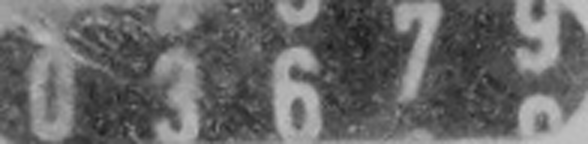
\includegraphics[width=\linewidth]{../assets/meter_gray.png}\\{\scriptsize gray}
    \end{center}\end{column}
    \begin{column}{0.25\textwidth}\begin{center}
      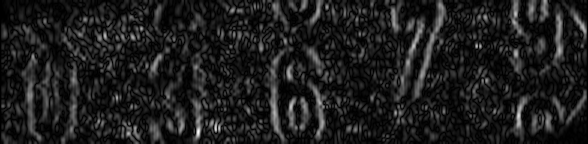
\includegraphics[width=\linewidth]{../assets/meter_sobelx.png}\\{\scriptsize $\partial x$ (vertical edges)}
    \end{center}\end{column}
    \begin{column}{0.25\textwidth}\begin{center}
      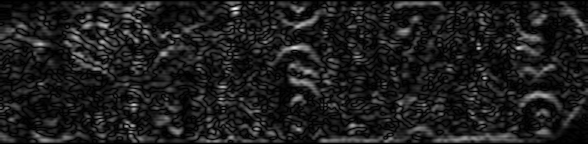
\includegraphics[width=\linewidth]{../assets/meter_sobely.png}\\{\scriptsize $\partial y$ (horizontal)}
    \end{center}\end{column}
    \begin{column}{0.25\textwidth}\begin{center}
      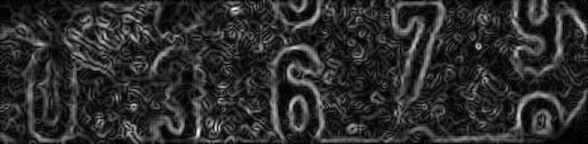
\includegraphics[width=\linewidth]{../assets/meter_sobelmag.png}\\{\scriptsize magnitude}
    \end{center}\end{column}
  \end{columns}
  \vspace{3pt}
  $x$-gradient highlights vertical strokes; $y$-gradient horizontal ones; magnitude combines both.
\end{frame}

\begin{frame}{Gradient magnitude \& direction}
  \begin{itemize}
    \item \term{Magnitude} $= \sqrt{g_x^2 + g_y^2}$: how strong the edge is (the bright edge map).
    \item \term{Direction} $= \operatorname{atan2}(g_y, g_x)$: which way intensity increases; the
          edge itself runs \emph{perpendicular} to this.
    \item Threshold the magnitude to get a binary edge map — but a fixed threshold is fragile.
  \end{itemize}
  \begin{badbox}
    Gradients are noise-sensitive: noise creates strong fake gradients. Always smooth first (Week 3/4).
  \end{badbox}
\end{frame}

\begin{frame}{Worked example: magnitude \& direction}
  Suppose at a pixel $g_x = 30$, $g_y = 40$.
  \begin{columns}[T]
    \begin{column}{0.55\textwidth}
      \begin{align*}
        |\nabla f| &= \sqrt{30^2 + 40^2} = \sqrt{2500} = \mathbf{50}\\[2pt]
        \theta     &= \operatorname{atan2}(40,30) \approx \mathbf{53^\circ}
      \end{align*}
      Gradient points up-and-right; the edge line runs at $53^\circ-90^\circ = -37^\circ$.
    \end{column}
    \begin{column}{0.45\textwidth}
      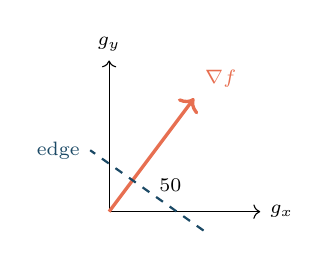
\begin{tikzpicture}[scale=0.6,font=\scriptsize]
        \draw[->] (0,0)--(3.2,0) node[right]{$g_x$};
        \draw[->] (0,0)--(0,3.2) node[above]{$g_y$};
        \draw[courseAccent,very thick,->] (0,0)--(1.8,2.4) node[above right]{$\nabla f$};
        \draw[coursePrimary,thick,dashed] (2.0,-0.4)--(-0.4,1.3) node[left]{edge};
        \node at (1.3,0.55){$50$};
      \end{tikzpicture}
    \end{column}
  \end{columns}
  \keyidea{Magnitude answers ``how strong?''; direction answers ``which way?'' — Canny needs both.}
\end{frame}

\begin{frame}[fragile]{Computing the gradient in OpenCV}
\begin{lstlisting}[language=Python]
gx = cv2.Sobel(gray, cv2.CV_64F, 1, 0, ksize=3)   # d/dx
gy = cv2.Sobel(gray, cv2.CV_64F, 0, 1, ksize=3)   # d/dy
mag  = cv2.magnitude(gx, gy)                       # sqrt(gx^2 + gy^2)
ang  = cv2.phase(gx, gy, angleInDegrees=True)      # direction
mag8 = cv2.convertScaleAbs(mag)                    # back to 0..255 for display
\end{lstlisting}
  \begin{badbox}
    Use a \emph{signed} type (\code{CV_64F}). On \code{uint8} the negative half of every edge is
    clipped to 0 — you lose one side of each edge.
  \end{badbox}
\end{frame}

\begin{frame}{The first-derivative family}
  \begin{center}
  \begin{tabular}{@{}llll@{}}
    \toprule
    \textbf{Operator} & \textbf{$x$-kernel} & \textbf{Idea} & \textbf{Notes} \\
    \midrule
    Roberts & $2{\times}2$ diagonal & diagonal diff & tiny, very noise-sensitive \\
    Prewitt & $[-1,0,1]$, equal rows & simple gradient & no centre weighting \\
    Sobel   & $[-1,0,1]$, rows $1,2,1$ & centre-weighted & the practical default \\
    Scharr  & rows $3,10,3$ & optimized $3{\times}3$ & better rotational accuracy \\
    \bottomrule
  \end{tabular}
  \end{center}
  \begin{columns}[T]
    \begin{column}{0.5\textwidth}
      \term{Prewitt-x}: $\begin{bmatrix}-1&0&1\\-1&0&1\\-1&0&1\end{bmatrix}$
    \end{column}
    \begin{column}{0.5\textwidth}
      \term{Scharr-x}: $\begin{bmatrix}-3&0&3\\-10&0&10\\-3&0&3\end{bmatrix}$
    \end{column}
  \end{columns}
  \vspace{2pt}
  \keyidea{They all estimate the same derivative; the weights trade noise-rejection for accuracy.}
\end{frame}

% ==================================================================
\section{Second derivative: Laplacian \& LoG}
% ==================================================================

\begin{frame}{Laplacian: the second derivative}
  \begin{columns}[T]
    \begin{column}{0.5\textwidth}
      \[\text{Laplacian }= \begin{bmatrix}0&1&0\\1&-4&1\\0&1&0\end{bmatrix}\]
      $\nabla^2 f = f_{xx} + f_{yy}$ — one kernel, sensitive to edges in \emph{all} directions.
    \end{column}
    \begin{column}{0.5\textwidth}\begin{center}
      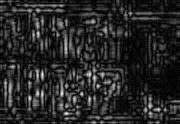
\includegraphics[width=0.9\linewidth]{../assets/plate_laplacian.png}\\{\scriptsize Laplacian of a plate}
    \end{center}\end{column}
  \end{columns}
  \vspace{3pt}
  \begin{itemize}
    \item Detects edges as \term{zero-crossings}: the 2nd derivative flips sign right at the edge.
    \item One kernel for every orientation — but even more noise-sensitive than the first derivative.
  \end{itemize}
\end{frame}

\begin{frame}{Zero-crossings: 1st vs 2nd derivative}
  \begin{center}
  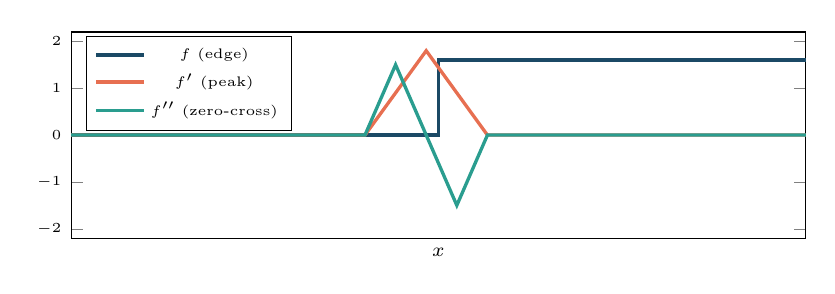
\begin{tikzpicture}
    \begin{axis}[width=0.9\linewidth,height=4.2cm,xlabel={$x$},
      xtick=\empty,ymin=-2.2,ymax=2.2,xmin=0,xmax=6,
      legend style={font=\tiny,at={(0.02,0.98)},anchor=north west},
      label style={font=\scriptsize},tick label style={font=\tiny}]
      \addplot[coursePrimary,very thick,const plot] coordinates
        {(0,0)(2.5,0)(3,1.6)(6,1.6)}; \addlegendentry{$f$ (edge)}
      \addplot[courseAccent,very thick] coordinates
        {(0,0)(2.4,0)(2.9,1.8)(3.4,0)(6,0)}; \addlegendentry{$f'$ (peak)}
      \addplot[courseGood,very thick] coordinates
        {(0,0)(2.4,0)(2.65,1.5)(2.9,0)(3.15,-1.5)(3.4,0)(6,0)}; \addlegendentry{$f''$ (zero-cross)}
    \end{axis}
  \end{tikzpicture}
  \end{center}
  \begin{itemize}
    \item First derivative: \term{peak} at the edge. Second derivative: \term{zero-crossing} at the edge.
    \item Finding a zero-crossing localizes the edge precisely — but you must smooth first.
  \end{itemize}
\end{frame}

\begin{frame}{LoG: Laplacian of Gaussian}
  \begin{itemize}
    \item Problem: the bare Laplacian screams at every noise pixel.
    \item Fix: \term{smooth with a Gaussian, then take the Laplacian} — the \term{LoG} operator.
    \item Because convolution is associative, this is \emph{one} pre-built kernel (the ``Mexican hat'').
  \end{itemize}
  \begin{mathbox}
    $\text{LoG} = \nabla^2 (G_\sigma * f) = (\nabla^2 G_\sigma) * f$. Bigger $\sigma$ $\Rightarrow$
    smoother, fewer/coarser edges. DoG (difference of two Gaussians) approximates it cheaply.
  \end{mathbox}
\end{frame}

\begin{frame}{Laplacian on the meter vs plate}
  \begin{columns}[T]
    \begin{column}{0.5\textwidth}\begin{center}
      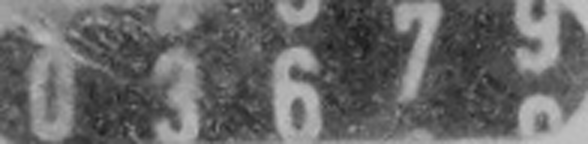
\includegraphics[width=0.55\linewidth]{../assets/meter_gray.png}\\{\scriptsize meter (gray)}\\[3pt]
      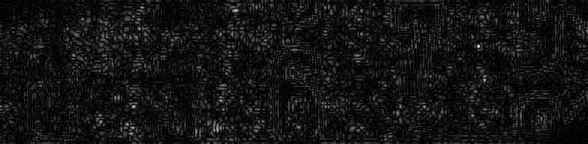
\includegraphics[width=0.55\linewidth]{../assets/meter_laplacian.png}\\{\scriptsize meter Laplacian}
    \end{center}\end{column}
    \begin{column}{0.5\textwidth}\begin{center}
      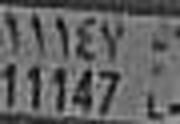
\includegraphics[width=0.7\linewidth]{../assets/plate_gray.png}\\{\scriptsize plate (gray)}\\[3pt]
      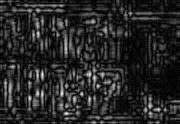
\includegraphics[width=0.7\linewidth]{../assets/plate_laplacian.png}\\{\scriptsize plate Laplacian}
    \end{center}\end{column}
  \end{columns}
  \vspace{2pt}
  Notice the double-edged (light/dark) ridges — the sign change straddling each real edge.
\end{frame}

% ==================================================================
\section{Noise \& why we smooth}
% ==================================================================

\begin{frame}{Why smooth before differentiating}
  \begin{itemize}
    \item Differentiation \term{amplifies} high frequencies — including noise.
    \item So the derivative of a noisy signal is dominated by noise, not edges.
    \item Smooth first (Gaussian), then differentiate — the basis of Sobel/Canny/LoG.
  \end{itemize}
  \begin{mathbox}
    Handy identity: (blur then differentiate) $=$ convolve with the \emph{derivative of the Gaussian},
    $\frac{d}{dx}(G_\sigma * f) = (\tfrac{d}{dx}G_\sigma) * f$ — one kernel does both.
  \end{mathbox}
\end{frame}

\begin{frame}{Noise turns into fake edges}
  \begin{columns}[T]
    \begin{column}{0.55\textwidth}
      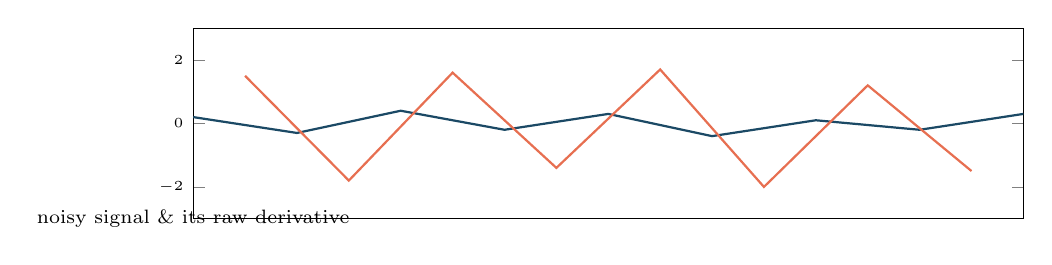
\begin{tikzpicture}
        \begin{axis}[width=\linewidth,height=4cm,title={noisy signal \& its raw derivative},
          xtick=\empty,xmin=0,xmax=8,ymin=-3,ymax=3,
          every axis title/.style={font=\scriptsize},
          label style={font=\scriptsize},tick label style={font=\tiny}]
          \addplot[coursePrimary,thick] coordinates
            {(0,0.2)(1,-0.3)(2,0.4)(3,-0.2)(4,0.3)(5,-0.4)(6,0.1)(7,-0.2)(8,0.3)};
          \addplot[courseAccent,thick] coordinates
            {(0.5,1.5)(1.5,-1.8)(2.5,1.6)(3.5,-1.4)(4.5,1.7)(5.5,-2.0)(6.5,1.2)(7.5,-1.5)};
        \end{axis}
      \end{tikzpicture}
    \end{column}
    \begin{column}{0.45\textwidth}
      \begin{itemize}
        \item The flat signal has small wobbles (noise).
        \item Its derivative (coral) swings wildly — every wobble looks like an ``edge''.
        \item A single Gaussian blur first flattens these before differentiating.
      \end{itemize}
    \end{column}
  \end{columns}
\end{frame}

% ==================================================================
\section{In-class exercise}
% ==================================================================

\begin{frame}{\faPen~In-class exercise (10 min)}
  \begin{infobox}[Reason about a 1D signal]
  \end{infobox}
  A row of pixels: \code{[10, 10, 10, 200, 200, 200]}.
  \begin{enumerate}
    \item Compute the first derivative as forward differences $f[i{+}1]-f[i]$. Where is it maximum?
    \item Apply the 1D kernel $[-1,0,1]$ (a mini Sobel-x) centred on each interior pixel. What is the peak value, and at which pixel?
    \item Now one pixel is noise: \code{[10,10,90,200,200,200]}. Recompute the differences — how big is the spurious response, and how would a blur reduce it?
  \end{enumerate}
\end{frame}

\begin{frame}{\faPen~Debrief}
  \begin{itemize}
    \item Differences: \code{[0,0,190,0,0]} — the derivative spikes at the $10\rightarrow200$ jump. That spike \emph{is} the edge.
    \item $[-1,0,1]$ centred at the pixel just left of the jump gives $200-10 = 190$: the peak lands on the edge.
    \item The noise pixel (90) makes differences \code{[0,80,110,0,0]}: a smaller, split response. A blur averages 90 back toward its neighbours before it becomes a false edge.
  \end{itemize}
  \keyidea{An edge is where the derivative is large. Everything today is a way to compute and clean that derivative.}
\end{frame}

% ==================================================================
\section{Practice notes}
% ==================================================================

\begin{frame}{Common pitfalls}
  \begin{badbox}[Don't differentiate raw, noisy pixels]
    A bare Laplacian or Sobel on an unsmoothed photo returns a speckled mess. Blur first.
  \end{badbox}
  \begin{badbox}[Don't clip the sign]
    Storing a gradient in \code{uint8} clips negatives to 0 — half of every edge vanishes.
    Use a signed type, then take $|\cdot|$ for display.
  \end{badbox}
\end{frame}

\begin{frame}{Good practice}
  \begin{goodbox}[Sensible defaults]
    Gaussian blur ($3{\times}3$ or $5{\times}5$) $\to$ Sobel \code{ksize=3} $\to$ magnitude.
    Reach for Scharr when a $3{\times}3$ Sobel looks direction-biased.
  \end{goodbox}
  \begin{goodbox}[Match the tool to the job]
    First derivative (Sobel) for edge \emph{strength/direction}; Laplacian/LoG when you want
    all-orientation response or precise zero-crossing locations.
  \end{goodbox}
\end{frame}

% ==================================================================
\section{Wrap-up}
% ==================================================================

\begin{frame}{What you should now be able to do}
  \begin{itemize}
    \item Explain an edge as a large gradient / a zero-crossing of the 2nd derivative.
    \item Compute Sobel-x/y by hand on a patch; get magnitude and direction.
    \item Compare Roberts/Prewitt/Sobel/Scharr and the Laplacian/LoG.
    \item Say why smoothing must come before differentiating.
  \end{itemize}
\end{frame}

\begin{frame}{Next session teaser}
  \begin{alertblock}{Session 2 — Canny \& clean contours}
    A thresholded Sobel magnitude is thick, broken and noisy. Next time we chain
    \term{smooth $\to$ gradient $\to$ non-maximum suppression $\to$ hysteresis} into the
    \term{Canny} detector — thin, connected, tunable edges — and connect them to the
    DocScan page finder.
  \end{alertblock}
  \begin{center}\small (No deliverable yet — bring your Sobel/Laplacian code from today.)\end{center}
\end{frame}

\begin{frame}[standout]
  An edge is where the derivative is large.\\[4pt]
  \normalsize Today: how to \emph{compute} that derivative and keep noise out of it.
\end{frame}

\end{document}
